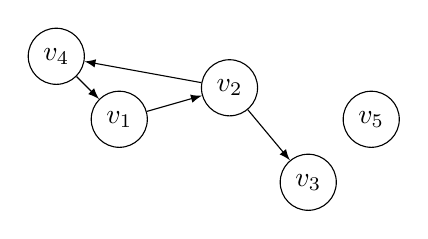
\begin{tikzpicture}[scale=0.8,mynode/.style=draw,circle,
                    goto/.style=->,>=latex]
\node[mynode] (v1) at (0,0) {$v_1$};
\node[mynode] (v2) at (1.75,0.5) {$v_2$};
\node[mynode] (v3) at (3,-1) {$v_3$};
\node[mynode] (v4) at (-1,1) {$v_4$};
\node[mynode] (v5) at (4,0) {$v_5$};
\draw[goto] (v1) -> (v2);
\draw[goto] (v4) -> (v1);
\draw[goto] (v2) -> (v4);
\draw[goto] (v2) -> (v3);
\draw[goto] (v5);
\end{tikzpicture}
